\textbf{Sigmoid neuron}, similarly to perceptron, has inputs $\vec{x}$ and weights. The key difference comes in once we inspect the output value and its calculation. Instead of perceptron's binary output 0 or 1, a sigmoid neuron outputs a real number between 0 and 1 using a \textit{sigmoid function}.\cite{nndl2015michaelnielsen}\cite{rojas2013neural}\cite{matous}

\begin{equation}
    {\sigma(\alpha) = \frac{1}{1 + e^{-\alpha}}}
\end{equation}

\begin{figure}[h]
	\centering
    \subfloat[\centering Step function]{{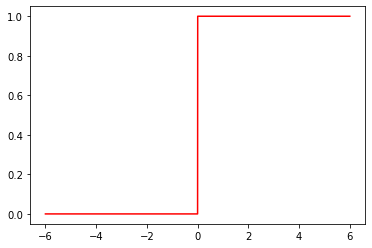
\includegraphics[width=6cm]{step}}}%
    \qquad
    \subfloat[\centering Sigmoid function]{{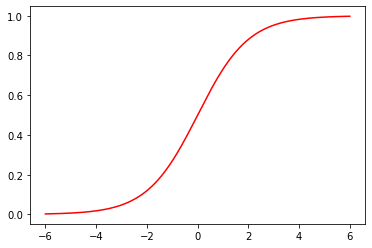
\includegraphics[width=6cm]{sigmoid}}}%
    \caption{Comparison between step function and sigmoid function}
\end{figure}
As shown in Figure 1.1, the sigmoid function(1.1a) is a smoothed-out version of the step function(1.1b).
